% ============================================================
% Oppgave 3
% ============================================================

\hypertarget{oppgave3}{}
\section*{Oppgave 3}
\addcontentsline{toc}{section}{Oppgave 3}
Filterets impulsrespons er:
\[
h[n]=\{1,3,2\}
\]
\subsection*{a)}
Dette er et FIR-filter. FIR står for \textit{Finite Impulse Response}. Impulsresponsen
består av et endelig antall verdier og blir null etter den tredje
verdien:
\[
h[n]=0,
\qquad n>2
\]
Filteret har heller ingen tilbakekobling fra tidligere
utgangsverdier.
\subsection*{b)}
Filteret består av tre grener fra inngangssignalet:
\begin{figure}[H]
    \centering
    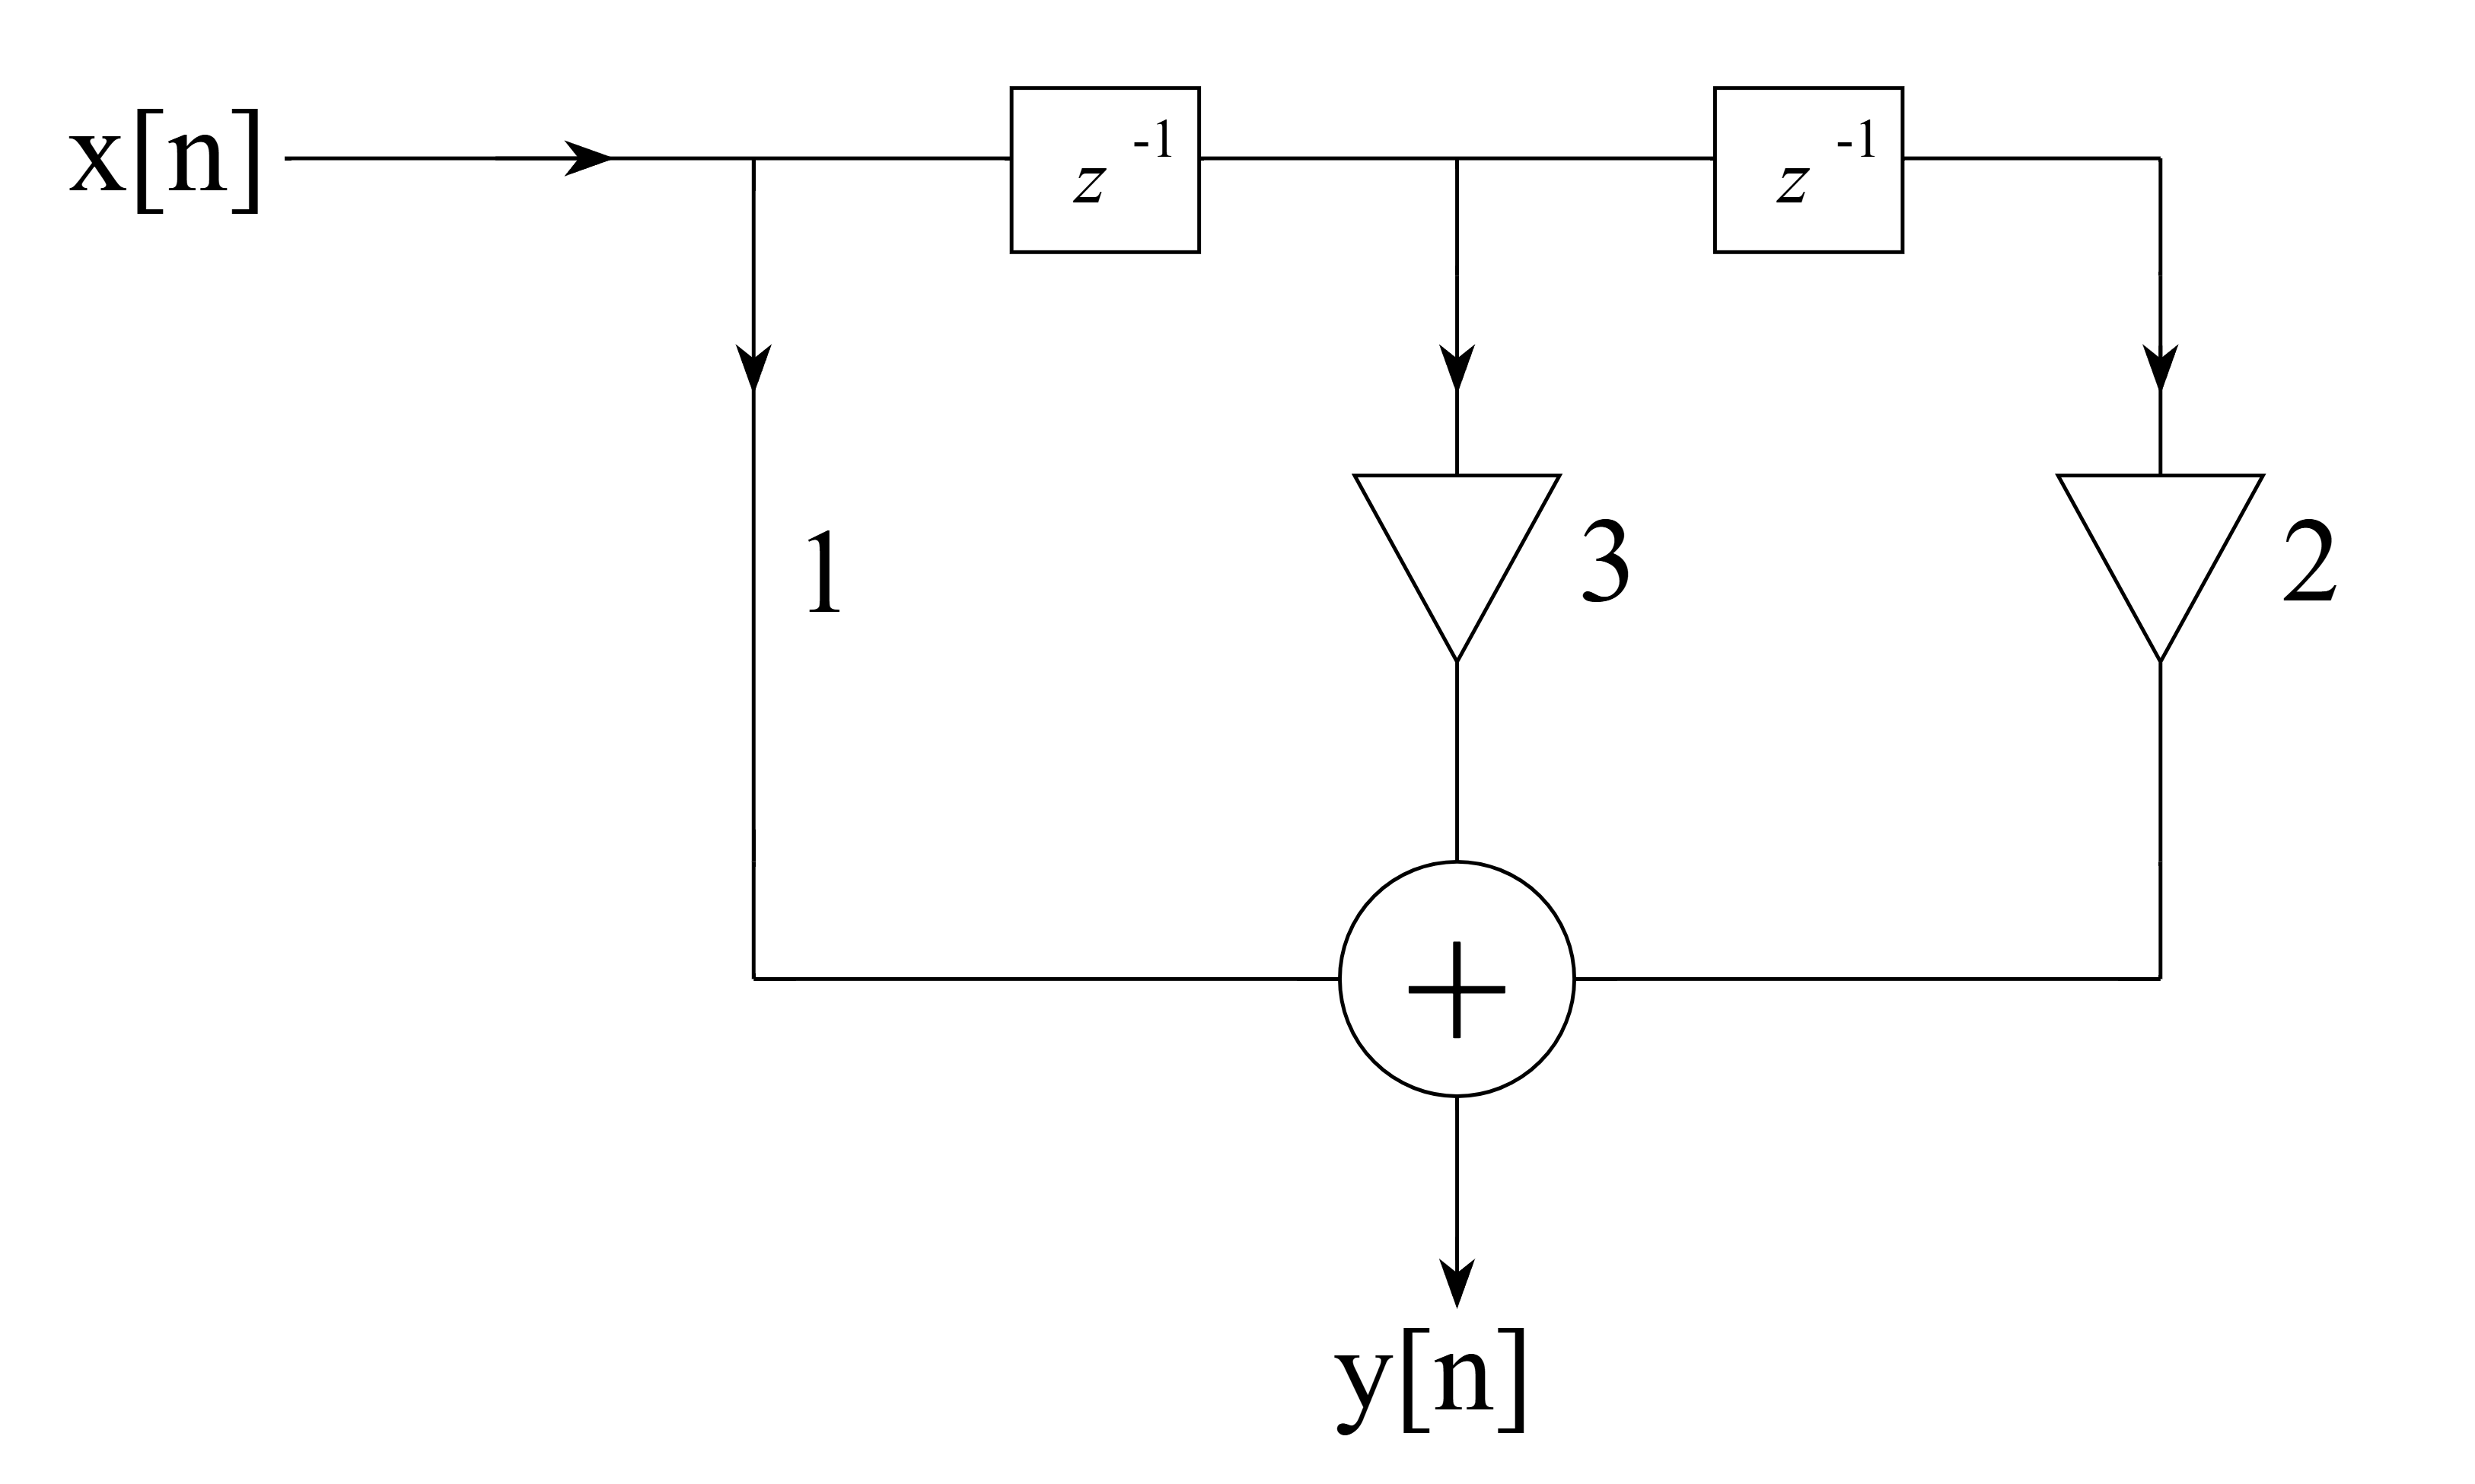
\includegraphics[width=0.9\textwidth]{../Media/fir1.png}
    \caption{FIR-filter struktur}
\end{figure}
De tre signalene som summeres er derfor:
\[
x[n], \qquad 3x[n-1], \qquad 2x[n-2]
\]
\subsection*{c)}
Differensligningen finnes direkte fra filterkoeffisientene:
\[
\boxed{
y[n]
=
x[n]
+
3x[n-1]
+
2x[n-2]
}
\]
\subsection*{d)}
Innsignalet er:
\[
x[n]=\{2,3,-1\}
\]
Utsignalet kan finnes ved konvolusjon:
\[
y[n]=x[n]*h[n]
\]
Dette gir:
\[
\{2,3,-1\}*\{1,3,2\}
=
\boxed{\{2,9,12,3,-2\}}
\]
\subsection*{e)}
Z-transformasjonen av impulsresponsen gir systemfunksjonen:
\[
H(z)
=
1+3z^{-1}+2z^{-2}
\]
Ved å multiplisere teller og nevner med $z^2$ får vi:
\[
H(z)
=
\frac{z^2+3z+2}{z^2}
\]
Telleren kan faktoriseres:
\[
z^2+3z+2
=
(z+1)(z+2)
\]
Systemfunksjonen blir dermed:
\[
\boxed{
H(z)
=
\frac{(z+1)(z+2)}{z^2}
}
\]
Nullpunktene er:
\[
z_1=-1,
\qquad
z_2=-2
\]
og filteret har en dobbeltpol i:
\[
z=0
\]
Figuren under viser pol-nullpunkts-diagrammet for FIR-filteret.
\begin{figure}[H]
    \centering
    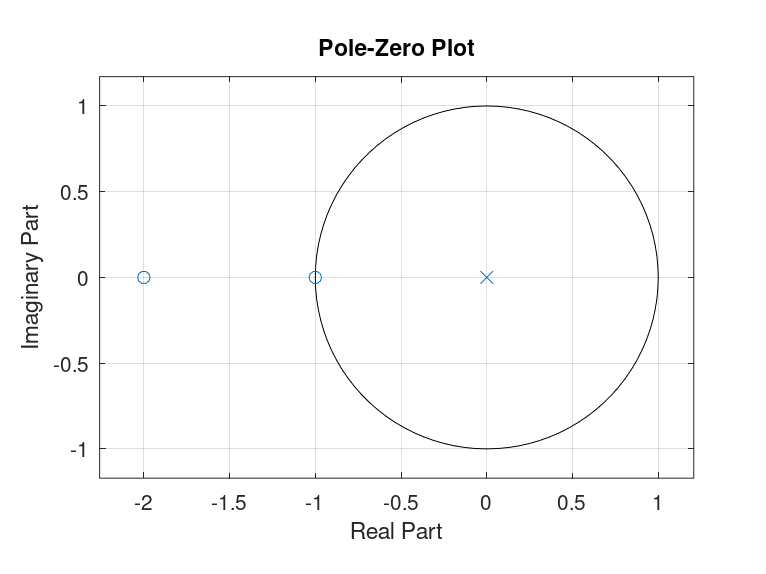
\includegraphics[width=0.9\textwidth]{../Media/polplot.png}
    \caption{Pol-nullpunkts-diagram for FIR-filteret}
\end{figure}